%!TEX root = ../../main.tex
% ============================================================
% 统计图表 / 条形统计图补全
% 本文件由 main.tex 通过 \input 引入，请勿单独编译
% 重构日期: 2026-04-11
% ============================================================

\subsection{解答：不完整统计图补全与样本推断}

\vspace{0.6cm}

\textbf{例 3 \quad 随着科技进步发展，在线学习已经成为部分人自主学习的选择。某校计划为学生提供以下四类学习方式：在线阅读、在线听课、在线答题和在线讨论。为了解学生的需求，该校随机对本校部分学生进行了“你对哪类在线学习方式最感兴趣的调查”，并根据调查结果绘制成两幅不完整的统计图（如图）。}

\vspace{0.4cm}

\textbf{（1）这次抽样调查的样本容量是 \underline{\makebox[1.5cm]{}}，在扇形统计图中“在线阅读”所在扇形圆心角的度数为 \underline{\makebox[1.5cm]{}}$^\circ$；\\
（2）将条形统计图补充完整；\\
（3）若该校共有学生 $1500$ 人，请你估计该校对“在线讨论”最感兴趣的学生人数。}

\vspace{0.4cm}
\textbf{解：}

\textbf{（1）} 由左侧条形图可知对“在线答题”最感兴趣的固定人数为 $\boldsymbol{18}$ 人，而对应的右侧扇形图中宣告其占据全体样本的 $\boldsymbol{20\%}$。\\
所以，本次抽样调查的总样本容量即可逆向求出： $18 \div 20\% = \boldsymbol{90}$（人）。\\
已知“在线阅读”组落座确切人数有 $\boldsymbol{24}$ 人，将该组占总体的比例映射入 $360^\circ$ 扇形圆盘体系，对应的扇形圆心角度数为：
$$360^\circ \times \frac{24}{90} = \boldsymbol{96^\circ}$$
\textbf{故，第一空应填：$\boldsymbol{90}$；第二空应填：$\boldsymbol{96}$。}

\vspace{0.4cm}

\textbf{（2）} 补充完整的条形统计图：\\
计算补充类别“在线听课”的实际空缺人数，即从大盘内减去已知三组：
$$90 - (24 + 18 + 12) = 90 - 54 = \boldsymbol{36}\text{（人）}$$
（注：条形统计图中绘制补充进度，见下方左侧图表中采用红色强调框限与色系高亮的再生条形柱。）

\vspace{0.4cm}

\begin{center}
\renewcommand{\arraystretch}{1.5}
\begin{tabular}{cc}
\begin{tikzpicture}[>=Stealth, x=1.5cm, y=0.08cm, baseline=(current bounding box.center)]
  % 绘制背景水平虚线网格
  \foreach \y in {6, 12, 18, 24, 30, 36, 42, 48} {
    \draw[gray!50, dashed, line width=0.5pt] (0, \y) -- (4.8, \y);
    \node[left, font=\footnotesize] at (0, \y) {\y};
  }
  \node[left, font=\footnotesize] at (0, 0) {$0$};

  % Y轴
  \draw[->, line width=0.8pt] (0, 0) -- (0, 56) node[above] {人数};
  % X轴
  \draw[->, line width=0.8pt] (0, 0) -- (5.2, 0) node[right] {方式};

  % 1. 在线阅读 (原有基柱)
  \fill[cyan!15, draw=black, line width=0.8pt] (1-0.3, 0) rectangle (1+0.3, 24);
  \node[above, font=\small] at (1, 24) {$24$};
  \node[below, align=center, font=\small] at (1, -1) {在线\\阅读};

  % 2. 在线听课 (新补推演数据，启用红色视觉最高级强调)
  \fill[red!15, draw=red, thick] (2-0.3, 0) rectangle (2+0.3, 36);
  \node[above, font=\small, text=red] at (2, 36) {\textbf{36}};
  \node[below, align=center, font=\small] at (2, -1) {在线\\听课};

  % 3. 在线答题 (原有核心桥梁基柱)
  \fill[cyan!15, draw=black, line width=0.8pt] (3-0.3, 0) rectangle (3+0.3, 18);
  \node[above, font=\small] at (3, 18) {$18$};
  \node[below, align=center, font=\small] at (3, -1) {在线\\答题};

  % 4. 在线讨论 (原有基柱)
  \fill[cyan!15, draw=black, line width=0.8pt] (4-0.3, 0) rectangle (4+0.3, 12);
  \node[above, font=\small] at (4, 12) {$12$};
  \node[below, align=center, font=\small] at (4, -1) {在线\\讨论};
\end{tikzpicture}
&
\begin{tikzpicture}[>=Stealth, line join=round, baseline=(current bounding box.center)]
  \def\R{2.1} % 控制扇形图物理半径
  \coordinate (O) at (0,0);
  
  % 根据推理事后严格切分并逆向复原原图圆心角版图
  % 1. 在线讨论: 12人占全身样本 48度 (恰好分布于 -90度直下线 到 -42度)
  \draw[fill=orange!15, draw=black, thick] (O) -- (-90:\R) arc (-90:-42:\R) -- cycle;
  \node[align=center, font=\small] at (-66:1.3) {在线\\讨论};

  % 2. 在线答题: 18人占 72度 (-42度 上升跨越死角到 30度)
  \draw[fill=yellow!20, draw=black, thick] (O) -- (-42:\R) arc (-42:30:\R) -- cycle;
  \node[align=center, font=\small] at (-6:1.3) {在线答题 \\ $20\%$};

  % 3. 在线听课: 36人豪占 144度 (30度 攀越天顶到达 174度)
  \draw[fill=red!5, draw=black, thick] (O) -- (30:\R) arc (30:174:\R) -- cycle;
  \node[align=center, font=\small] at (102:1.3) {在线听课};

  % 4. 在线阅读: 24人占 96度 (从 174度 归拢闭合至的南极点 270度/-90度)
  \draw[fill=cyan!15, draw=black, thick] (O) -- (174:\R) arc (174:270:\R) -- cycle;
  \node[align=center, font=\small] at (222:1.3) {在线\\阅读};

\end{tikzpicture}
\\
\textbf{补充后的条形统计图} & \textbf{原理还原的扇形统计图}
\end{tabular}
\end{center}

\vspace{0.4cm}

\textbf{（3）} 估计该校对“在线讨论”最感兴趣的学生人数：\\
由抽样样本比对可知，选择“在线讨论”的发生频率为 $\displaystyle\frac{12}{90} = \frac{2}{15}$。\\
由于样本具有极高的代表性，利用样本局部频率同化估计全校人口总体，其估算人数规模为：
$$1500 \times \frac{2}{15} = \boldsymbol{200}\text{（人）}$$
\textbf{答：} 由统计推断，估计该校中对“在线讨论”最感兴趣的学生群体规模大约有 $200$ 人。

\vspace{0.6cm}

{\small\color{blue!70!black}
\textbf{画图及逻辑控制思路解构：}\\
\textbf{1. 中继参数锚定与宏观体量双推机制：} 搞定一切棘手的双图信息残缺残破题（即数据学界内的“桥梁题”），最致命的核心打法准则是永远去寻找那个**“既在条形表里有着孤立数值量纲、又能在圆盘图里对应确确实实准确百分比的那个‘基石节点’”**。本题唯一的突破口破局枢纽就是且仅有“在线答题”（人数 $18$ 与统筹占比 $20\%$并存）；抓到它，只需一发顺向除法就能在一瞬间如探囊取物般破译出被命题组强行封锁隐藏的最大系统总体盘池容量（$90$ 人）。进而犹如摧枯拉朽的多米诺骨牌般顺藤摸瓜，横扫算出扇形其余缺失的夹角参数，并依靠总池减法最终补上缺漏条形图的 $36$ 个窟窿数位！\\
\textbf{2. 逆向复刻简化解析法与相片级原版图纸重建工程：} 在指令底层要求对右侧原图圆盘执行再造与全息代码推翻重画时，程序严格启动了比对原图象形阵列中的墨丘利分布方位机制：我们精准审视到了原出题图片底稿里“在线阅读”和“在线讨论”区划下方那道不留情面的大裂谷直立切割缝——它赫然垂直，地坐落于 $Y$ 轴南端也就是 $-90^\circ$ 位置！以此敏锐的参照物确立为零度偏转法向起锚点，顺时针反哺逆推、严实塞入用上述运算得到的每一个度数间片（$48^\circ, 72^\circ, 144^\circ$ 及最终收死归零接壤第一道缝的 $96^\circ$）。由此一举在脱离任何外部包的情形下依靠纯 Latex 内核图形编译器实现了这幅带着精密透视感的终极矢量复刻。
}

%% ==============================
%% 第14题（题7）：区间频数分布直方图与补全推断
%% ==============================
\newpage

\newpage

\subsection{解答：图书类别条形统计图补全与扇形统计图}

\vspace{0.6cm}

\textbf{\LARGE 42.} \textbf{（8 分）某中学准备购进一批图书供学生阅读，为了合理配备各类图书，从全体学生中随机抽取了部分学生进行了问卷调查。问卷设置了五种选项：A"艺术类"，B"文学类"，C"科普类"，D"体育类"，E"其他类"。每名学生必须且只能选择其中最喜爱的一类图书，将调查结果整理绘制成如下两幅不完整的统计图。}

\vspace{0.4cm}
\textbf{解：}

\textbf{（1）解题分析：}

由扇形统计图知 B 占 $20\%$，条形图中 B $= 20$ 人，故抽样总数 $= 20 \div 20\% = 100$ 人。

D 的人数 $= 100 - 10 - 20 - 40 - 5 = 25$ 人。

\vspace{0.2cm}
\textbf{（2）补全条形统计图：}

\begin{center}
{\textbf{学生最喜爱图书类别的人数条形统计图}}
\end{center}

\vspace{0.1cm}
\begin{center}
\begin{tikzpicture}[>=Stealth]
  % 缩放参数
  \def\xstep{1.2}   % 每组间距
  \def\ystep{0.12}   % Y轴每人高度，40人=4.8cm
  \def\barw{0.7}     % 柱宽

  % 1. Y轴与X轴
  \draw[thick, black, ->] (0,0) -- (0, 42*\ystep + 0.5) node[left, font=\normalsize] {人数/名};
  \draw[thick, black, ->] (0,0) -- (6*\xstep + 0.3, 0);

  % 2. Y轴刻度标签（仅标签，不画虚线）
  \foreach \y in {5, 10, 15, 20, 25, 30, 35, 40} {
      \node[left, font=\small] at (0, \y*\ystep) {\y};
  }
  \node[left, font=\small] at (0, 0) {0};

  % 3. 条形柱（先绘制，虚线后绘制以覆盖在上层）
  % A = 10（艺术类）
  \fill[gray!35] (1*\xstep - \barw/2, 0) rectangle (1*\xstep + \barw/2, 10*\ystep);
  \draw[thick, black] (1*\xstep - \barw/2, 0) rectangle (1*\xstep + \barw/2, 10*\ystep);
  \node[above, font=\small\bfseries] at (1*\xstep, 10*\ystep) {10};

  % B = 20（文学类）
  \fill[gray!35] (2*\xstep - \barw/2, 0) rectangle (2*\xstep + \barw/2, 20*\ystep);
  \draw[thick, black] (2*\xstep - \barw/2, 0) rectangle (2*\xstep + \barw/2, 20*\ystep);
  \node[above, font=\small\bfseries] at (2*\xstep, 20*\ystep) {20};

  % C = 40（科普类）
  \fill[gray!35] (3*\xstep - \barw/2, 0) rectangle (3*\xstep + \barw/2, 40*\ystep);
  \draw[thick, black] (3*\xstep - \barw/2, 0) rectangle (3*\xstep + \barw/2, 40*\ystep);
  \node[above, font=\small\bfseries] at (3*\xstep, 40*\ystep) {40};

  % D = 25（体育类，补全项，红色标注）
  \fill[gray!35] (4*\xstep - \barw/2, 0) rectangle (4*\xstep + \barw/2, 25*\ystep);
  \draw[thick, black] (4*\xstep - \barw/2, 0) rectangle (4*\xstep + \barw/2, 25*\ystep);
  \node[above, font=\small\bfseries, text=red] at (4*\xstep, 25*\ystep) {25};

  % E = 5（其他类）
  \fill[gray!35] (5*\xstep - \barw/2, 0) rectangle (5*\xstep + \barw/2, 5*\ystep);
  \draw[thick, black] (5*\xstep - \barw/2, 0) rectangle (5*\xstep + \barw/2, 5*\ystep);
  \node[above, font=\small\bfseries] at (5*\xstep, 5*\ystep) {5};

  % 4. 水平虚线——从Y轴延伸到对应条形柱左边缘即截止
  % y=10 → A柱 (x=1*xstep)
  \draw[dashed, gray!70] (0, 10*\ystep) -- (1*\xstep - \barw/2, 10*\ystep);
  % y=20 → B柱 (x=2*xstep)
  \draw[dashed, gray!70] (0, 20*\ystep) -- (2*\xstep - \barw/2, 20*\ystep);
  % y=40 → C柱 (x=3*xstep)
  \draw[dashed, gray!70] (0, 40*\ystep) -- (3*\xstep - \barw/2, 40*\ystep);
  % y=25 → D柱 (x=4*xstep)
  \draw[dashed, gray!70] (0, 25*\ystep) -- (4*\xstep - \barw/2, 25*\ystep);
  % y=5 → E柱 (x=5*xstep)
  \draw[dashed, gray!70] (0, 5*\ystep) -- (5*\xstep - \barw/2, 5*\ystep);

  % 5. X轴标签
  \foreach \x/\label in {1/A, 2/B, 3/C, 4/D, 5/E} {
      \node[below, font=\normalsize] at (\x*\xstep, -0.15) {\label};
  }
  \node[below, font=\normalsize] at (6*\xstep, -0.15) {类别};

\end{tikzpicture}
\end{center}

\vspace{0.4cm}
\textbf{（3）各问作答：}

\begin{itemize}
    \item[\textbf{(1)}] 抽样总数 $= 20 \div 20\% = \underline{\textcolor{red}{\,100\,}}$ 人。

    D 的人数 $= 100 - 10 - 20 - 40 - 5 = 25$ 人，条形统计图已补全。

    \item[\textbf{(2)}] A"艺术类"所对应的圆心角 $= 360^\circ \times \dfrac{10}{100} = \underline{\textcolor{red}{\,36\,}}^\circ$。

    \item[\textbf{(3)}] 估计喜爱 C"科普类"图书的学生人数 $= 1200 \times \dfrac{40}{100} = \underline{\textcolor{red}{\,480\,}}$ 人。
\end{itemize}

\vspace{0.4cm}
{\small\color{blue!70!black}
\textbf{绘图原理与步骤：}\\
\textbf{1. 坐标系：} 开放式直角坐标系（双轴带箭头）。Y 轴 $0$--$40$，每 $5$ 人一条水平虚线。X 轴 5 组类别 + "类别"标签。缩放参数 \texttt{\textbackslash{}xstep=1.2}，\texttt{\textbackslash{}ystep=0.12}，\texttt{\textbackslash{}barw=0.7}。\\
\textbf{2. 条形柱：} \texttt{gray!35} 浅灰填充 + 黑色描边。补全项 D 的数值用红色标注。\\
\textbf{3. 数据推导：} B 占 $20\% = 20$ 人 $\Rightarrow$ 总数 $100$。D $= 100 - 10 - 20 - 40 - 5 = 25$。A 圆心角 $= 360^\circ \times 10\% = 36^\circ$。
}

%% ==============================
%% 第52题（补充题）：Rt△ABC 中线、尺规作图与菱形证明
%% ==============================
\newpage

\newpage

\subsection{解答：BMI 条形统计图补全与计算}

\vspace{0.6cm}

\textbf{\LARGE 44.} \textbf{（12 分）国际上常用体质指数 BMI（Body Mass Index）衡量人体胖瘦程度，其计算公式是}
$$\text{BMI} = \frac{\text{体重}}{\text{身高}^2} \quad \text{（体重单位：kg，身高单位：m）}$$

\textbf{中国成人的 BMI 数值与体重的关系为：BMI $< 18.5$ 为体重过低；$18.5 \leqslant$ BMI $< 24$ 为体重正常；$24 \leqslant$ BMI $< 28$ 为超重；BMI $\geqslant 28$ 为肥胖。某健身馆随机抽取了一部分顾客的身高体重数据，计算得到他们的 BMI 值并绘制了两幅不完整的统计图。}

\vspace{0.4cm}
\textbf{解：}

\textbf{（1）解题分析：}

由扇形统计图知体重正常占 $35\%$，条形图中体重正常 $= 7$ 人，

故抽样总数 $= 7 \div 35\% = 20$ 人。

超重人数 $= 20 - 2 - 7 - 3 = 8$ 人。

\vspace{0.2cm}
\textbf{（2）补全条形统计图：}

\begin{center}
{\textbf{抽取的员工体重情况的条形统计图}}
\end{center}

\vspace{0.1cm}
\begin{center}
\begin{tikzpicture}[>=Stealth]
  % 缩放参数
  \def\xstep{1.4}   % 每组间距（4个类别较宽标签）
  \def\ystep{0.4}   % Y轴每人高度，10人=4cm
  \def\barw{0.8}    % 柱宽

  % 1. Y轴与X轴（朴素黑色，无虚线）
  \draw[thick, black, ->] (0,0) -- (0, 11*\ystep + 0.3) node[left, font=\normalsize] {人数};
  \draw[thick, black, ->] (0,0) -- (5*\xstep + 0.3, 0);

  % 2. Y轴刻度标签（仅标签，不画虚线）
  \foreach \y in {2, 4, 6, 8, 10} {
      \node[left, font=\small] at (0, \y*\ystep) {\y};
      \draw[thin, black] (-0.08, \y*\ystep) -- (0, \y*\ystep);  % 短刻度线
  }
  \node[left, font=\small] at (0, 0) {0};

  % 3. 条形柱（朴素黑色描边，白色/浅灰填充）
  % 体重过低 = 2
  \fill[white] (1*\xstep - \barw/2, 0) rectangle (1*\xstep + \barw/2, 2*\ystep);
  \draw[thick, black] (1*\xstep - \barw/2, 0) rectangle (1*\xstep + \barw/2, 2*\ystep);
  \node[above, font=\small\bfseries] at (1*\xstep, 2*\ystep) {2};

  % 体重正常 = 7
  \fill[white] (2*\xstep - \barw/2, 0) rectangle (2*\xstep + \barw/2, 7*\ystep);
  \draw[thick, black] (2*\xstep - \barw/2, 0) rectangle (2*\xstep + \barw/2, 7*\ystep);
  \node[above, font=\small\bfseries] at (2*\xstep, 7*\ystep) {7};

  % 超重 = 8（补全项，红色标注）
  \fill[white] (3*\xstep - \barw/2, 0) rectangle (3*\xstep + \barw/2, 8*\ystep);
  \draw[thick, black] (3*\xstep - \barw/2, 0) rectangle (3*\xstep + \barw/2, 8*\ystep);
  \node[above, font=\small\bfseries, text=red] at (3*\xstep, 8*\ystep) {8};

  % 肥胖 = 3
  \fill[white] (4*\xstep - \barw/2, 0) rectangle (4*\xstep + \barw/2, 3*\ystep);
  \draw[thick, black] (4*\xstep - \barw/2, 0) rectangle (4*\xstep + \barw/2, 3*\ystep);
  \node[above, font=\small\bfseries] at (4*\xstep, 3*\ystep) {3};

  % 4. X轴标签（中文标签）
  \node[below, font=\small] at (1*\xstep, -0.1) {体重};
  \node[below, font=\small] at (1*\xstep, -0.5) {过低};
  \node[below, font=\small] at (2*\xstep, -0.1) {体重};
  \node[below, font=\small] at (2*\xstep, -0.5) {正常};
  \node[below, font=\small] at (3*\xstep, -0.3) {超重};
  \node[below, font=\small] at (4*\xstep, -0.3) {肥胖};
  \node[below, font=\normalsize] at (5*\xstep, -0.3) {类别};

\end{tikzpicture}
\end{center}

\vspace{0.4cm}
\textbf{（3）各问作答：}

\begin{itemize}
    \item[\textbf{(1)}] 抽取了 $\underline{\textcolor{red}{\,20\,}}$ 名顾客。

    （$7 \div 35\% = 20$）

    \item[\textbf{(2)}] 条形统计图已补全（超重 $= 20 - 2 - 7 - 3 = 8$ 人）。

    \item[\textbf{(3)}] 体重"肥胖"所对应的扇形圆心角 $= 360^\circ \times \dfrac{3}{20} = \underline{\textcolor{red}{\,54\,}}^\circ$。

    \item[\textbf{(4)}] 小张身高 $1.80$ m，BMI 值为 $27$。

    当前体重 $= 27 \times 1.80^2 = 27 \times 3.24 = 87.48$ kg。

    体重正常要求 BMI $< 24$，即体重 $< 24 \times 1.80^2 = 24 \times 3.24 = 77.76$ kg。

    至少需要减掉 $87.48 - 77.76 = 9.72$ kg，精确到 $1$ kg，

    即至少需要减掉 $\underline{\textcolor{red}{\,10\,}}$ kg。
\end{itemize}

\vspace{0.4cm}
{\small\color{blue!70!black}
\textbf{绘图原理与步骤：}\\
\textbf{1. 坐标系：} 开放式直角坐标系（双轴带箭头），朴素黑色配色，不使用虚线。Y 轴 $0$--$10$，仅在偶数刻度处标注数值和短刻度线。X 轴 4 个类别标签 + "类别"。缩放参数 \texttt{\textbackslash{}xstep=1.4}，\texttt{\textbackslash{}ystep=0.4}，\texttt{\textbackslash{}barw=0.8}。\\
\textbf{2. 条形柱：} 白色填充 + 黑色描边（朴素风格）。补全项"超重"的数值用红色标注。\\
\textbf{3. 数据推导：} 体重正常占 $35\% = 7$ 人 $\Rightarrow$ 总数 $20$。超重 $= 20 - 2 - 7 - 3 = 8$。肥胖圆心角 $= 360^\circ \times 15\% = 54^\circ$。减重 $= 27 \times 3.24 - 24 \times 3.24 = 9.72 \approx 10$ kg。
}

%% ==============================
%% 第54题（补充题）：体育成绩等级条形统计图
%% ==============================
\newpage

\newpage

\subsection{解答：体育成绩等级条形统计图补全}

\vspace{0.6cm}

\textbf{\LARGE 45.} \textbf{（12 分）某校组织七年级学生体育健康抽测（满分为 100 分），七年级（1）班 25 名学生的成绩统计如下：}

90，74，88，65，98，76，81，42，85，70，55，80，95，88，72，87，61，56，76，66，78，72，82，63，100。

\textbf{（1）90 分及以上为 A 级，75$\sim$89 分为 B 级，60$\sim$74 分为 C 级，60 分以下为 D 级。请把下面表格补充完整，并将图中的条形图补充完整。}

\vspace{0.3cm}
\textbf{解：}

\textbf{数据分类统计：}

\begin{itemize}
    \item A 级（$\geqslant 90$）：90，98，95，100 $\Rightarrow$ \textcolor{red}{4} 人
    \item B 级（75$\sim$89）：88，76，81，85，80，88，87，76，78，82 $\Rightarrow$ \textcolor{red}{10} 人
    \item C 级（60$\sim$74）：74，65，70，72，61，66，72，63 $\Rightarrow$ 8 人
    \item D 级（$< 60$）：42，55，56 $\Rightarrow$ \textcolor{red}{3} 人
\end{itemize}

验证：$4 + 10 + 8 + 3 = 25$ $\checkmark$

\vspace{0.3cm}
\textbf{补全表格：}

\begin{center}
\renewcommand{\arraystretch}{1.4}
\begin{tabular}{c|c|c|c|c}
\noalign{\hrule height 1.2pt}
等级 & A & B & C & D \\
\hline
人数 & \textcolor{red}{4} & \textcolor{red}{10} & 8 & \textcolor{red}{3} \\
\noalign{\hrule height 1.2pt}
\end{tabular}
\end{center}

\vspace{0.3cm}
\textbf{补全条形统计图：}

\begin{center}
\begin{tikzpicture}[>=Stealth]
  % 缩放参数
  \def\xstep{1.2}   % 每组间距
  \def\ystep{0.4}   % Y轴每人高度，10人=4cm
  \def\barw{0.7}    % 柱宽

  % 1. Y轴与X轴
  \draw[thick, black, ->] (0,0) -- (0, 11*\ystep + 0.3) node[left, font=\normalsize] {人数};
  \draw[thick, black, ->] (0,0) -- (5*\xstep + 0.3, 0);

  % 2. Y轴刻度标签（每1人一个刻度）
  \foreach \y in {1, 2, 3, 4, 5, 6, 7, 8, 9, 10} {
      \node[left, font=\small] at (0, \y*\ystep) {\y};
      \draw[thin, black] (-0.06, \y*\ystep) -- (0, \y*\ystep);  % 短刻度线
  }
  \node[left, font=\small] at (0, 0) {0};

  % 3. 条形柱（白色填充 + 黑色描边）
  % A = 4（补全项，红色标注）
  \fill[white] (1*\xstep - \barw/2, 0) rectangle (1*\xstep + \barw/2, 4*\ystep);
  \draw[thick, black] (1*\xstep - \barw/2, 0) rectangle (1*\xstep + \barw/2, 4*\ystep);
  \node[above, font=\small\bfseries, text=red] at (1*\xstep, 4*\ystep) {4};

  % B = 10（补全项，红色标注）
  \fill[white] (2*\xstep - \barw/2, 0) rectangle (2*\xstep + \barw/2, 10*\ystep);
  \draw[thick, black] (2*\xstep - \barw/2, 0) rectangle (2*\xstep + \barw/2, 10*\ystep);
  \node[above, font=\small\bfseries, text=red] at (2*\xstep, 10*\ystep) {10};

  % C = 8（已有项）
  \fill[white] (3*\xstep - \barw/2, 0) rectangle (3*\xstep + \barw/2, 8*\ystep);
  \draw[thick, black] (3*\xstep - \barw/2, 0) rectangle (3*\xstep + \barw/2, 8*\ystep);
  \node[above, font=\small\bfseries] at (3*\xstep, 8*\ystep) {8};

  % D = 3（补全项，红色标注）
  \fill[white] (4*\xstep - \barw/2, 0) rectangle (4*\xstep + \barw/2, 3*\ystep);
  \draw[thick, black] (4*\xstep - \barw/2, 0) rectangle (4*\xstep + \barw/2, 3*\ystep);
  \node[above, font=\small\bfseries, text=red] at (4*\xstep, 3*\ystep) {3};

  % 4. 水平虚线——从Y轴到对应柱左边缘，在柱上层
  % y=4 → A柱 (x=1*xstep)
  \draw[dashed, gray!70] (0, 4*\ystep) -- (1*\xstep - \barw/2, 4*\ystep);
  % y=10 → B柱 (x=2*xstep)
  \draw[dashed, gray!70] (0, 10*\ystep) -- (2*\xstep - \barw/2, 10*\ystep);
  % y=8 → C柱 (x=3*xstep)
  \draw[dashed, gray!70] (0, 8*\ystep) -- (3*\xstep - \barw/2, 8*\ystep);
  % y=3 → D柱 (x=4*xstep)
  \draw[dashed, gray!70] (0, 3*\ystep) -- (4*\xstep - \barw/2, 3*\ystep);

  % 5. X轴标签
  \foreach \x/\label in {1/A, 2/B, 3/C, 4/D} {
      \node[below, font=\normalsize] at (\x*\xstep, -0.15) {\label};
  }
  \node[below, font=\normalsize] at (5*\xstep, -0.15) {等级};

\end{tikzpicture}
\end{center}

\vspace{0.4cm}
\textbf{（2）} 60 分以上为合格，合格人数 $= 4 + 10 + 8 = 22$ 人。

估计七年级合格人数 $= 1000 \times \dfrac{22}{25} = \underline{\textcolor{red}{\,880\,}}$ 人。

\vspace{0.3cm}
\textbf{（3）} 应选择\textbf{扇形统计图}，因为扇形统计图能清晰地表示出各等级人数占总人数的百分比。

各等级百分比：A 级 $= \dfrac{4}{25} = 16\%$，B 级 $= \dfrac{10}{25} = 40\%$，C 级 $= \dfrac{8}{25} = 32\%$，D 级 $= \dfrac{3}{25} = 12\%$。

\vspace{0.3cm}
\begin{center}
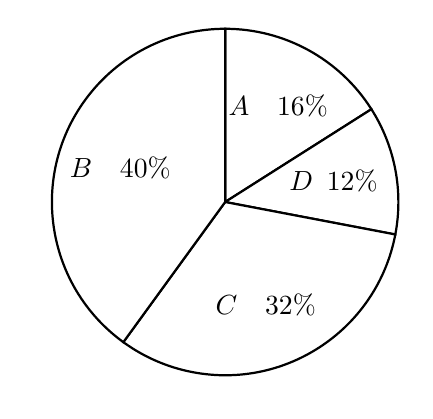
\begin{tikzpicture}
  % 扇形统计图参数
  \def\radius{2.2}

  % 扇形角度计算（从 90° 顺时针）：
  % A = 16% → 57.6°   起始 90°   结束 32.4°
  % D = 12% → 43.2°   起始 32.4° 结束 -10.8°
  % C = 32% → 115.2°  起始 -10.8° 结束 -126°
  % B = 40% → 144°    起始 -126°  结束 -270°(=90°)

  % 1. 绘制扇形（从顶部 90° 开始，顺时针：A → D → C → B）
  % A 扇区 (16%)：90° → 32.4°
  \fill[white] (0,0) -- (90:\radius) arc (90:32.4:\radius) -- cycle;
  \draw[thick, black] (0,0) -- (90:\radius) arc (90:32.4:\radius) -- cycle;

  % D 扇区 (12%)：32.4° → -10.8°
  \fill[white] (0,0) -- (32.4:\radius) arc (32.4:-10.8:\radius) -- cycle;
  \draw[thick, black] (0,0) -- (32.4:\radius) arc (32.4:-10.8:\radius) -- cycle;

  % C 扇区 (32%)：-10.8° → -126°
  \fill[white] (0,0) -- (-10.8:\radius) arc (-10.8:-126:\radius) -- cycle;
  \draw[thick, black] (0,0) -- (-10.8:\radius) arc (-10.8:-126:\radius) -- cycle;

  % B 扇区 (40%)：-126° → -270°(=90°)
  \fill[white] (0,0) -- (-126:\radius) arc (-126:-270:\radius) -- cycle;
  \draw[thick, black] (0,0) -- (-126:\radius) arc (-126:-270:\radius) -- cycle;

  % 2. 扇区标签（居中放置在各扇区中间角度方向）
  % A：中间角度 = (90+32.4)/2 = 61.2°
  \node[font=\normalsize] at (61.2:1.4) {$A$\quad $16\%$};

  % D：中间角度 = (32.4+(-10.8))/2 = 10.8°
  \node[font=\normalsize] at (10.8:1.4) {$D$\enspace $12\%$};

  % C：中间角度 = (-10.8+(-126))/2 = -68.4°
  \node[font=\normalsize] at (-68.4:1.4) {$C$\quad $32\%$};

  % B：中间角度 = (-126+(-270))/2 = -198°
  \node[font=\normalsize] at (-198:1.4) {$B$\quad $40\%$};

\end{tikzpicture}
\end{center}

\vspace{0.4cm}
{\small\color{blue!70!black}
\textbf{绘图原理与步骤：}\\
\textbf{1. 坐标系：} 开放式直角坐标系（双轴带箭头）。Y 轴 $0$--$10$，每 $1$ 人一个刻度及短刻度线。X 轴 4 个等级标签 + "等级"。缩放参数 \texttt{\textbackslash{}xstep=1.2}，\texttt{\textbackslash{}ystep=0.4}，\texttt{\textbackslash{}barw=0.7}。\\
\textbf{2. 条形柱：} 白色填充 + 黑色描边。已知 C $= 8$，补全项 A/B/D 用红色标注。\\
\textbf{3. 虚线：} 每个柱顶对应一条水平虚线，从 Y 轴延伸到该柱左边缘截止，绘制在柱上层。\\
\textbf{4. 表格：} 使用 \texttt{\textbackslash{}noalign\{\textbackslash{}hrule height 1.2pt\}} 加粗上下边框，内部用 \texttt{\textbackslash{}hline} 标准线。\\
\textbf{5. 数据统计：} 逐个分类 25 个成绩，A $= 4$$、$B $= 10$$、$C $= 8$$、$D $= 3$。
}

%% ==============================
%% 第55题（补充题）：月总销售额条形统计图补全
%% ==============================
\newpage

\newpage

\subsection{解答：月总销售额条形统计图补全}

\vspace{0.6cm}

\textbf{\LARGE 46.} \textbf{（例 1）某人工智能科技公司 2025 年 8—12 月各月总销售额及"智能机器人"类产品的各月销售额占比分别如图所示。已知该公司 2025 年 8—12 月总销售额共为 200 万元，观察统计图（图 6.6.1，图 6.6.2），解答下列问题：}

\vspace{0.4cm}
\textbf{解：}

\textbf{（1）解题分析：}

$8$--$12$ 月总销售额共 $200$ 万元，已知 $8$ 月 $= 35, 9$ 月 $= 45, 10$ 月 $= 30, 12$ 月 $= 50$。

$11$ 月销售额 $= 200 - 35 - 45 - 30 - 50 = 40$ 万元。

\vspace{0.2cm}
\textbf{补全条形统计图：}

\begin{center}
{\textbf{各月总销售额条形统计图}}
\end{center}

\vspace{0.1cm}
\begin{center}
\begin{tikzpicture}[>=Stealth]
  % 缩放参数
  \def\xstep{1.2}   % 每月间距
  \def\ystep{0.08}   % Y轴每万元高度，50万=4cm
  \def\barw{0.7}     % 柱宽

  % 1. Y轴与X轴
  \draw[thick, black, ->] (0,0) -- (0, 55*\ystep + 0.3) node[left, font=\small] {月总销售额/万元};
  \draw[thick, black, ->] (0,0) -- (6*\xstep + 0.3, 0);

  % 2. Y轴刻度标签（每10万一个）
  \foreach \y in {10, 20, 30, 40, 50} {
      \node[left, font=\small] at (0, \y*\ystep) {\y};
      \draw[thin, black] (-0.06, \y*\ystep) -- (0, \y*\ystep);
  }
  \node[left, font=\small] at (0, 0) {0};

  % 4. 水平虚线——从Y轴到对应柱左边缘，在柱上层
  % y=35 → 8月柱 (x=1*xstep)
  \draw[dashed, gray!70] (0, 35*\ystep) -- (1*\xstep - \barw/2, 35*\ystep);
  % y=45 → 9月柱 (x=2*xstep)
  \draw[dashed, gray!70] (0, 45*\ystep) -- (2*\xstep - \barw/2, 45*\ystep);
  % y=30 → 10月柱 (x=3*xstep)
  \draw[dashed, gray!70] (0, 30*\ystep) -- (3*\xstep - \barw/2, 30*\ystep);
  % y=40 → 11月柱 (x=4*xstep)
  \draw[dashed, gray!70] (0, 40*\ystep) -- (4*\xstep - \barw/2, 40*\ystep);
  % y=50 → 12月柱 (x=5*xstep)
  \draw[dashed, gray!70] (0, 50*\ystep) -- (5*\xstep - \barw/2, 50*\ystep);

  % 3. 条形柱（灰色填充 + 黑色描边）
  % 8月 = 35
  \fill[gray!35] (1*\xstep - \barw/2, 0) rectangle (1*\xstep + \barw/2, 35*\ystep);
  \draw[thick, black] (1*\xstep - \barw/2, 0) rectangle (1*\xstep + \barw/2, 35*\ystep);
  \node[above, font=\small\bfseries] at (1*\xstep, 35*\ystep) {35};

  % 9月 = 45
  \fill[gray!35] (2*\xstep - \barw/2, 0) rectangle (2*\xstep + \barw/2, 45*\ystep);
  \draw[thick, black] (2*\xstep - \barw/2, 0) rectangle (2*\xstep + \barw/2, 45*\ystep);
  \node[above, font=\small\bfseries] at (2*\xstep, 45*\ystep) {45};

  % 10月 = 30
  \fill[gray!35] (3*\xstep - \barw/2, 0) rectangle (3*\xstep + \barw/2, 30*\ystep);
  \draw[thick, black] (3*\xstep - \barw/2, 0) rectangle (3*\xstep + \barw/2, 30*\ystep);
  \node[above, font=\small\bfseries] at (3*\xstep, 30*\ystep) {30};

  % 11月 = 40（补全项，红色标注）
  \fill[gray!35] (4*\xstep - \barw/2, 0) rectangle (4*\xstep + \barw/2, 40*\ystep);
  \draw[thick, black] (4*\xstep - \barw/2, 0) rectangle (4*\xstep + \barw/2, 40*\ystep);
  \node[above, font=\small\bfseries, text=red] at (4*\xstep, 40*\ystep) {40};

  % 12月 = 50
  \fill[gray!35] (5*\xstep - \barw/2, 0) rectangle (5*\xstep + \barw/2, 50*\ystep);
  \draw[thick, black] (5*\xstep - \barw/2, 0) rectangle (5*\xstep + \barw/2, 50*\ystep);
  \node[above, font=\small\bfseries] at (5*\xstep, 50*\ystep) {50};



  % 5. X轴标签
  \foreach \x/\label in {1/8, 2/9, 3/10, 4/11, 5/12} {
      \node[below, font=\normalsize] at (\x*\xstep, -0.15) {\label};
  }
  \node[below, font=\normalsize] at (6*\xstep, -0.15) {月份};

\end{tikzpicture}
\end{center}

\vspace{0.4cm}
\textbf{（2）判断哪个月"智能机器人"销售额最高：}

各月"智能机器人"销售额 $=$ 月总销售额 $\times$ 占比：

\begin{center}
\renewcommand{\arraystretch}{1.4}
\begin{tabular}{c|c|c|c|c|c}
\noalign{\hrule height 1.2pt}
月份 & 8 月 & 9 月 & 10 月 & 11 月 & 12 月 \\
\hline
总销售额（万元） & 35 & 45 & 30 & 40 & 50 \\
\hline
占比 & 20\% & 15\% & 18\% & 25\% & 22\% \\
\hline
销售额（万元） & 7 & 6.75 & 5.4 & 10 & \textcolor{red}{11} \\
\noalign{\hrule height 1.2pt}
\end{tabular}
\end{center}

\vspace{0.2cm}
$12$ 月"智能机器人"类产品的销售额最高，为 $50 \times 22\% = \underline{\textcolor{red}{\,11\,}}$ 万元。

理由：虽然 $11$ 月占比最高（$25\%$），但 $12$ 月总销售额最大（$50$ 万元），$50 \times 22\% = 11$ 万元 $> 40 \times 25\% = 10$ 万元。

\vspace{0.4cm}
{\small\color{blue!70!black}
\textbf{绘图原理与步骤：}\\
\textbf{1. 坐标系：} 开放式直角坐标系（双轴带箭头）。Y 轴 $0$--$50$，每 $10$ 万一个刻度。X 轴 5 个月份标签 + "月份"。缩放参数 \texttt{\textbackslash{}xstep=1.2}，\texttt{\textbackslash{}ystep=0.08}，\texttt{\textbackslash{}barw=0.7}。\\
\textbf{2. 条形柱：} \texttt{gray!35} 浅灰填充 + 黑色描边。补全项 $11$ 月用红色数值标注。\\
\textbf{3. 虚线：} 每个柱顶对应一条水平虚线从 Y 轴到柱左边缘，绘制在柱上层。\\
\textbf{4. 数据推导：} 总计 $200$ 万 $\Rightarrow$ $11$ 月 $= 200 - 35 - 45 - 30 - 50 = 40$。各月"智能机器人"销售额 $=$ 总额 $\times$ 占比，$12$ 月 $11$ 万最高。
}

%% ==============================
%% 第56题（补充题）：数学实验——几何概型（蒙特卡洛方法）
%% ==============================
\newpage
